

%\begin{itemize}
%	\item Is it possible to avoid the baseline problem?
%	\item Define services in terms of performance, not characteristics.
%	\end{itemize}
%Product definition(suggestions):
%		\begin{itemize}
%			\item fast response product (gets paid for delivering in full as fast as possible, over short time horizons)
%			\item sustained delivery product (gets paid for the time period it is able to fully deliver the service)
%		\end{itemize}
% AS on the aggregators/DERs terms (new requirements)\\ 
%Verification and Settlement

\bondy{1) Ideal ancillary services needs are established and product performance is directly derived from these needs in form of a scalar heuristic based on performance variables. % are directly related to the system need. % (not upon minimum requirements).
2) remuneration based upon optimal value of the scalar heuristic.
3) New service definition leads to a new market clearing mechanism.}

The ideal source for ancillary service is one with ``unlimited capabilities in terms of response time, energy output, ability to frequently reverse their output, ability to respond and follow the AGC setpoint changes, and size .''\cite{makarov2008assessing}\footnote{For this kind of response to be optimal, changes must be made to the AGC algorithm \cite{peydayesh2012effects}.} In order to include and give incentive to the participation of technologies that in some parameters are closer to the ideal than those defined by the current service and market requirements, two methods can be utilized: product differentiation or product restructuring.

Some transmission system operators, like PJM, have already introduced the idea that better service performance is more valuable\footnote{See RegA and RegD in [cite].}, and split their regulation market into slow service product and a fast service product. 

This work explores the alternative, that is, restructuring the market, such that all technologies can participate in the same market, and the system operator can optimize the use of the resources based upon their capabilities. This entails reformulating the temporal and market requirements, and removing the requirements that implicitly assume that the services are provided by traditional generators, thus making the requirements technology agnostic.

The new service requirements definitions

- PRIM derived from inertia and no overshoot beyond settling frequency \& duration derived from secondary response \\
-- dimensioning of primary reserve defines settling frequency

- SECO derived from (cost/resource-optimal) primary and desired frequency restoration time 

- TERT derived from time to response

%It is concluded in \cite{makarov2008assessing} that a generator providing ancillary services close to the ideal (i.e. with large ramping rates), are more efficient for arresting frequency excursions earlier, and are therefore more valuable. There is a system wide benefit in creating better market opportunities for fast responsive resources. But in some instances, units that are able to provide very fast responses are not able to sustain their response for the currently required length of time (\textcolor{red}{refer to Vestas example if published, or other relevant example}).\bondy{To do: This whole paragraph should be reformulated so that the parameters are more generic, according to the service} Therefore the value of a unit should not only be evaluated based upon its ramping time, but also its response endurance. This paper proposes a new way of expressing these two service requirements into a single value. 

\subsection{Service Performance Parametrization}
Resource model: 

 - PROPOSAL1: ramp rate (MW/min), delay(min), duration (min), power (MW)\\
 
VOLUME:  (duration-(delay+power/ramp))*power+1/2*power/ramp*power)
 
- PERF: RMSE(Ideal unit parameters - parameters of the volume brick)
 
 - PROPOSAL2: full response time, duration, power\\
 
 alpha1*duration + alpha2*power - alpha3*

\bondy{We need express the system needs through parameters. Bring in Figure 3 or similar}\\
indicators

defining perfectly (responding) resource characterization

"threshold response" - the minimally acceptable reserve provisions (the reserve need)



\subsection{Performance-based Remuneration}

\subsection{Service Procurement Process}
\textit{Step 1:} Ancillary service specification by System operator. A system operator defines the system requirements and objectives for a specific ancillary service. These requirements are primarily formulated in terms of minimum requirements for the overall response. 

\textit{Step 2:} (AS) Service tender conditions: 
The tender defines requested total service volume, bid parameters and a derived performance parameter $\kappa$. 

The bid parameters are service-specific and serve both for market-clearing and performance calculation. The parameters are chosen considering idealized response characteristics, simplicity of calculations, service needs, verifiability, (linearity?) \kh{[...tbd...] }
The performance parameter defines the trade-off between bid parameters. 

Also, the tender will specify the granularity of the bids, so there is a standard bid size, e.g. 1 kW, of which each player can bid several of. For example, if aggregator \emph{X} wants to sell 5 MW, it bids 5000 units of the service. In this way, each bid's performance value $\kappa$, and the parameters that conforms it, will be comparable.

Steps 1-2 apply define the market setup. Steps 3-7 apply to each tendering period. 

\textit{Step 3:} Bid formulation:
AS aggregator bids submitted include: 
\begin{itemize}
\item offered service parameters
\item bid price
\item (for cross-validation) estimated $\kappa$
\item unit quantity (volume)
\end{itemize}


\textit{Step 4:} Market Clearing: based on submitted bids and required procurement volume the market is cleared by incrementally increasing the pool. For each new block of bids added to the portfolio, a new tetris optimization is done by the TSO. When the minimum requirements to the service specifications is met, the market is finished/cleared.

outcome: procured reserve portfolio; market clearing price according to the highest cleared price.

[\textit{Step 5: }Activation]

[\textit{Step 6:} Verification]

\textit{Step 7:} Remuneration is based on the market clearing price and the performance parameter $\kappa$. 
$\$*volume * \kappa - penalty$
penalty if Bid specs not met according to validation.


\textit{rationale:} \\
a) clearing at marginal cost provides correct competitive incentives [cite?Nordic market]; 

b) removal of 'minimum' requirements facilitates market liquidity, removing barriers for demand response participation;

c) performance-based remuneration favours better service \kh{[ahrr -this is so obvious, i can't find the words]};

d) bid formulation uses simplified constraints that can be addressed both for conventional generation and are also straightforward to be formulated as response capability of a diverse DR portfolio;

e) Steps 5 \& 6 out of scope/do not require revision.




\subsection{Proposal for Market Structure and Clearing}

In order to clear the market, all bids are sorted into a merit order list (price vs. volume), and the TSO will select from cheapest to most expensive the bids that covers its needed spectrum of $\kappa$ values. \kara{I don't think $\kappa$ is introduced before.}

%At the same time, demand response (DR) has shown to be capable of very fast ramping times \textcolor{red}{[cite:Vrettos-Powertech,Changhong Zhao-Caltech (Jason attended his talk) others?...]} which leads to arresting frequency excursions faster and at higher nadir. But for the foreseeable future traditional generators will still be delivering most of the ancillary services, and therefore the requirements must encompass the capabilities of both both slow reacting and fast reacting units. We therefore propose that the performance requirements are defined as a band, where the lower bound is the minimum acceptable service delivery, and the upper bound is represented by the optimal (hence by definition the maximum achievable) response.

%There are few of the current requirements that already measure performance (Table~\ref{tab:requirements}).% For primary frequency control, the change in operating point according to the frequency deviation $\Delta_P$, as well as the controller insensitivity (dead-band) are two parameters that describe the performance of the service.


%Definition of services in term of the droop dead-band and the shape of the slopes of the droop.
%
%Requirements that make sense:
%\begin{itemize}
%\item Primary frequency control
%\begin{itemize}
%\item Dead band
%\item Full delivery within \emph{x} time (could be a curve as proposed by Eto)
%\item ``droop'' (call it something different)
%\end{itemize}
%\begin{itemize}
%\item Deployment start
%\item Full delivery/availability
%\end{itemize}
%\end{itemize}
%
%I propose, to use the Integral Square Error index (as in my ISGT paper) and define the requirements as minimum and optimal bands. Depending on how we define the error, the quadratic nature of the ISE will emphasize punishment of performance close to the acceptable limits, or emphasize reward of performance close to the ideal.

%\begin{equation}
%\Delta P_G(t) = - \frac{1}{f_n S_G}\Delta f_m (t) P_{G,n}.\label{eq:droop}
%\end{equation}
%For primary frequency response, the optimal response is formulated from the optimal droop, following the equation:
%and the frequency dead-band. The minimum response requirement is given in base of the how long the generator has to give the maximum output (established by Eq.~\eqref{eq:droop}). Also, a probabilistic term could be added, such that 95 percentile respects the requirements. The response would be a linear transformation of the frequency deviation (Figure~\ref{fig:primarydroopresponse})
%\begin{figure}[ht!]
%\centering
%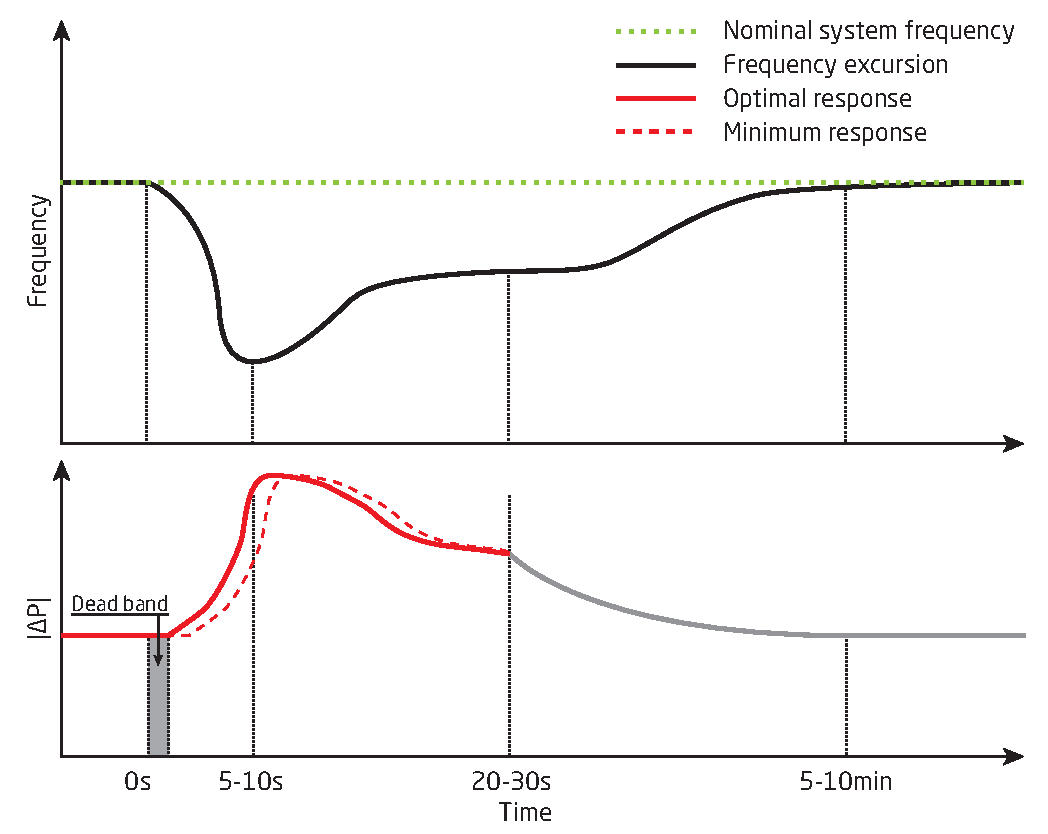
\includegraphics[width=1\columnwidth]{primary_frequency_control.pdf}
%\caption{Power response of a primary frequency control providing unit with perfect frequency following and with a droop of 4\%.}
%\label{fig:primarydroopresponse}
%\end{figure}
%
%Another way of formulating the optimal response is in terms of the rise time of the response (Figure~\ref{fig:primarytimeresponse})\cite{eto2010use}.
%\begin{figure}[ht!]
%\centering
%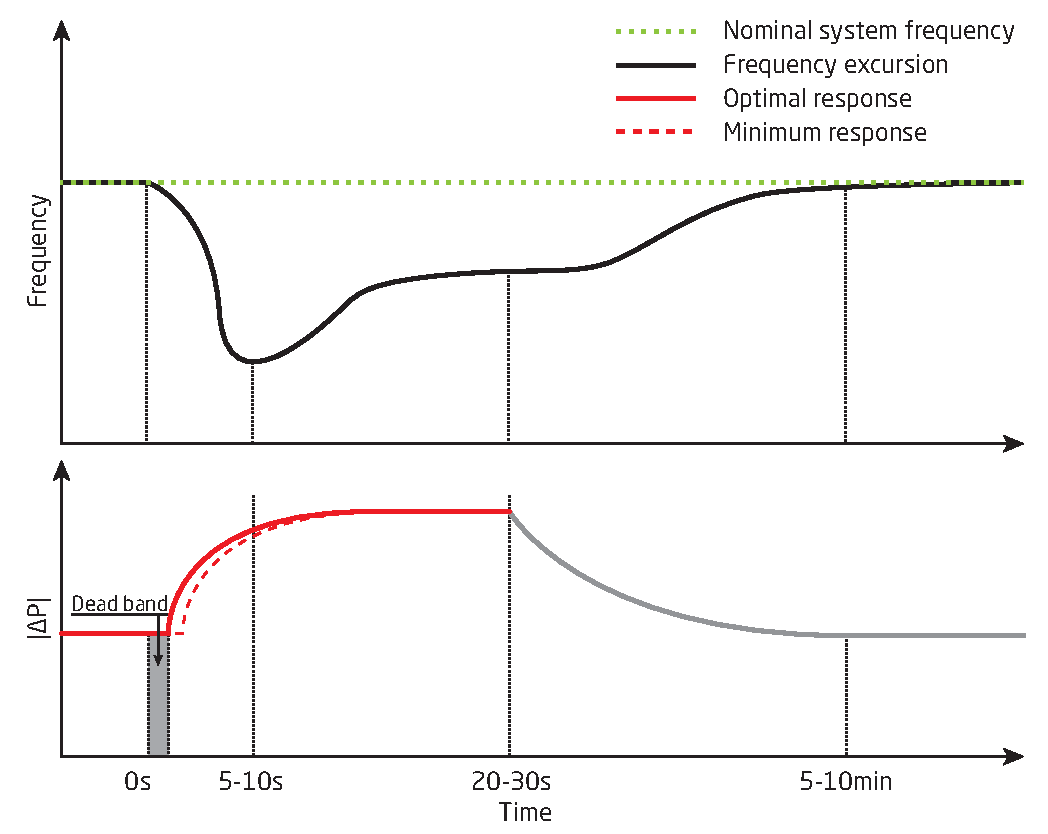
\includegraphics[width=1\columnwidth]{primary_frequency_control2.pdf}
%\caption{Power response of a primary frequency control providing unit when full delivery must be achieved within a time frame.}
%\label{fig:primarytimeresponse}
%\end{figure}
%
%For the secondary frequency control, the optimal response is formulated as a step function, or near step function because a response that is too steep could cause system instability. As in primary frequency control, the limits are defined by the allowable delay and a probabilistic term (Figure~\ref{fig:secondarytimeresponse}).
%\begin{figure}[ht!]
%\centering
%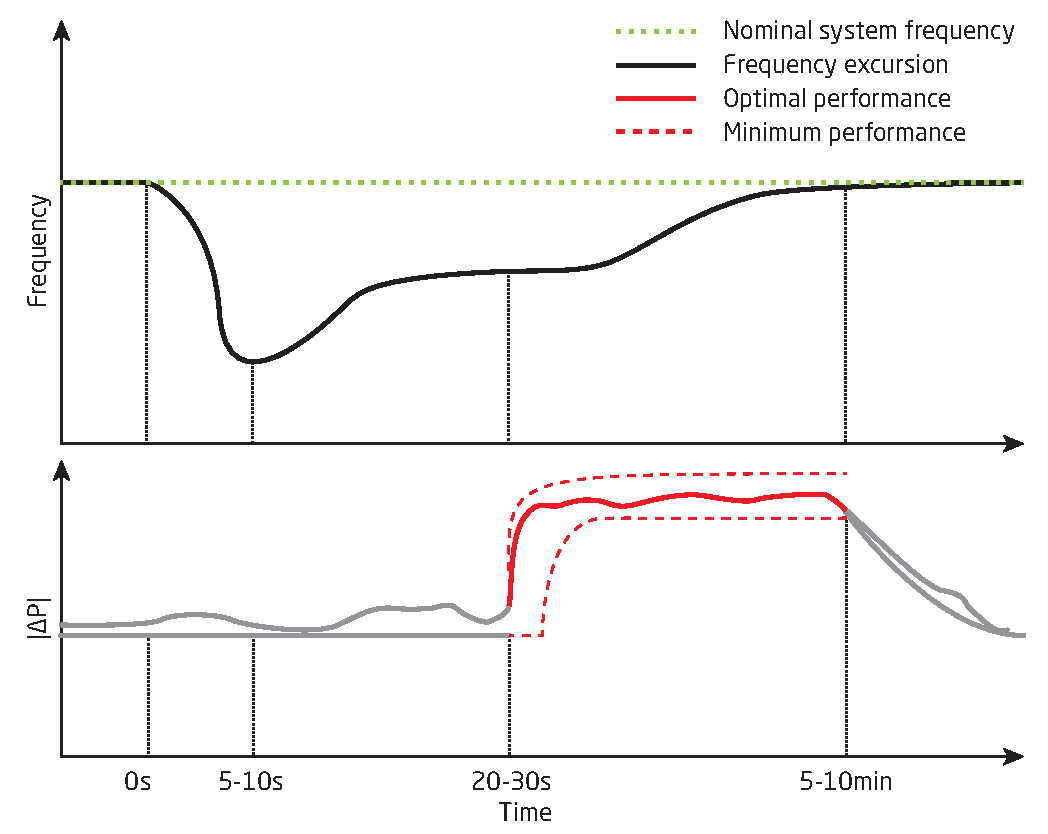
\includegraphics[width=1\columnwidth]{secondary_frequency_control2.pdf}
%\caption{Power response of a unit providing secondary frequency control indicating a time frame in which full delivery must be achieved.}
%\label{fig:secondarytimeresponse}
%\end{figure}
%We have identified three categories of requirements for ancillary services: performance requirements, unit specification requirements and market requirements.
%
%For primary frequency control the classification is the following:
%
%\emph{Performance requirements:} 
%\begin{itemize}
%\item Full availability
%\item Deployment end *
%\item Frequency characteristic
%\end{itemize}
%
%\emph{Unit specification requirements:}
%\begin{itemize}
%\item Droop of generator
%\item Compulsory adjustable droop
%\item Accuracy of frequency measurements
%\item controller insensitivity
%\item full deployment before a deviation of \emph{X} frequency
%\item Accuracy of SCADA measurements **
%\end{itemize}
%
%\emph{Market specification requirements:}
%\begin{itemize}
%\item Minimum reserve/bid size
%\item Contract \emph{X} time before delivery
%\item Bid symmetry
%\item Combined delivery
%\end{itemize}
%
%For secondary frequency control the classification is the following:
%
%\emph{Performance requirements:} 
%\begin{itemize}
%\item Deployment start
%\item Full availability
%\item Deployment end *
%\end{itemize}
%
%\emph{Unit specification requirements:}
%\begin{itemize}
%\item Control architecture
%\item Accuracy of frequency measurement
%\item Exchanges measurement
%\item Controller cycle time
%\item Controller type (P-term and I-term if applicable)
%\item K-factor for measuring ACE
%\item Accuracy of SCADA measurements **
%\end{itemize}
%
%\emph{Market specification requirements:}
%\begin{itemize}
%\item Minimum bid size
%\item Contract \emph{X} time before delivery
%\item Bid symmetry
%\item Combined delivery
%\item Bid duration
%\end{itemize}
%
%For tertiary frequency control the classification is the following:
%
%\emph{Performance requirements:}
%\begin{itemize}
%\item Deployment start
%\item Full availability
%\item Deployment end\textcolor{red}{(not sure on this one, since in many cases it is a rescheduling)}
%\end{itemize}
%
%\emph{Unit specification requirements:}
%\begin{itemize}
%\item Accuracy of SCADA measurements **
%\end{itemize}
%
%\emph{Market specification requirements:}
%\begin{itemize}
%\item Minimum bid size
%\item Contract \emph{X} time before delivery
%\item Bid symmetry
%\item Combined delivery
%\item Bid duration
%\end{itemize}